\documentclass{article}
\usepackage{amsmath}
\usepackage{amssymb}
\usepackage{enumitem}
\usepackage{algorithm}
\usepackage{listings}
\usepackage{color,xcolor}
\usepackage[T1]{fontenc}
\usepackage{fontawesome}
\usepackage{etoolbox}
\usepackage{multicol}
\usepackage{geometry}
\usepackage[colorlinks=true,linkcolor=blue,urlcolor=red,bookmarksopen=true]{hyperref}
\usepackage{tikz, pgfplots, tkz-euclide,calc}
    \usetikzlibrary{patterns,snakes,shapes.arrows,3d,patterns.meta,angles,quotes}
    \geometry{
        total = {160mm, 237mm},
        left = 25mm,
        right = 35mm,
        top = 30mm,
        bottom = 30mm,
      }
\usepackage{physics}
\usepackage{ifthen}
\usepackage[outline]{contour} % glow around text
\tikzset{>=latex} % for LaTeX arrow head
\contourlength{1.2pt}
\colorlet{myred}{red!65!black}
\tikzstyle{ground}=[preaction={fill,top color=black!10,bottom color=black!5,shading angle=20},
                    fill,pattern=north east lines,draw=none,minimum width=0.3,minimum height=0.6]
\tikzstyle{mass}=[line width=0.6,red!30!black,fill=red!40!black!10,rounded corners=1,
                  top color=red!40!black!20,bottom color=red!40!black!10,shading angle=20]
\tikzstyle{mass shadow}=[line width=0.6,rounded corners=1,loosely dashed]
\tikzstyle{rope}=[brown!70!black,line width=1.2,line cap=round] %very thick

% FORCES SWITCH
\tikzstyle{force}=[->,myred,thick,line cap=round]
\tikzstyle{Fproj}=[force,myred!40]
\newcommand{\vbF}{\vb{F}}
\newboolean{showforces}
\setboolean{showforces}{true}

\usepackage{tcolorbox}
     \tcbuselibrary{listings,skins}

\newcommand{\enter}{\raisebox{-1.8pt}{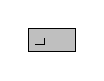
\begin{tikzpicture}[scale=0.3]
    \draw[thin,fill=lightgray] (0,0) rectangle (2,1);
    \draw (0.3,0.3) -- (0.7,0.3)--(0.7,0.6);     
\end{tikzpicture}}}

\definecolor{HIMAmuda}{HTML}{01D1FD}
\definecolor{HIMAtua}{HTML}{02016A}
\definecolor{HIMAabu}{HTML}{CBCBCC}
\definecolor{pgray}{rgb}{0.5,0.5,0.5}
\definecolor{pblue}{rgb}{0.13,0.13,1}
\definecolor{pgreen}{rgb}{0,0.5,0}
\definecolor{pred}{rgb}{0.9,0,0}
\definecolor{pgrey}{rgb}{0.46,0.45,0.48}
\definecolor{pcyan}{HTML}{D4EFFC}
\definecolor{lblue}{HTML}{00AEEF}
\definecolor{input}{HTML}{AAE1FA}
\definecolor{bg}{rgb}{0.95, 0.95, 0.92}
\definecolor{vscode}{HTML}{282A36}
\definecolor{PastelGreen}{HTML}{77DD77}

\newcommand{\inputscan}[1]{\raisebox{0pt}[1pt]{\colorbox{darkgray}{#1}}}

\usepackage{listings}

\lstdefinestyle{Liang}{
language=Java,
showspaces=false,
showtabs=false,
breaklines=true,
showstringspaces=false,
breakatwhitespace=true,
commentstyle=\color{pgray},
keywordstyle=\color{pblue},
stringstyle=\color{pgreen},
basicstyle=\small\ttfamily,
frame=single,
backgroundcolor=\color{pcyan},
escapeinside={(*}{*)},}

\lstdefinestyle{output}{
    language=Java,
    backgroundcolor=\color{vscode},
    basicstyle=\small\ttfamily\color{white},
    frame=none,
    escapeinside={(*}{*)},
    showspaces=false,
    showtabs=false,
    breaklines=true,
    showstringspaces=false,
    breakatwhitespace=true,
    keywordstyle=\color{white},
    }

\lstdefinestyle{standard}{
    language=Java,
    showspaces=false,
    showtabs=false,
    breaklines=true,
    showstringspaces=false,
    breakatwhitespace=true,
    commentstyle=\color{pgray},
    keywordstyle=\color{pblue},
    stringstyle=\color{pgreen},
    basicstyle=\small\ttfamily,
    frame=single,
    backgroundcolor=\color{bg},
    escapeinside={(*}{*)},}
\lstset{style=Liang}

\newtcblisting{RunCode}[1][enhanced,drop shadow]{
    arc=0pt, outer arc=0pt,
    boxsep=1pt,
    boxrule=2pt,
    auto outer arc,
    colback=vscode,
    colframe=bg,
    listing only, 
    listing style=output,
    title=\color{black}Ex. Output,
    #1
    }
\newtcblisting{RunCodeMore}[1][enhanced,drop shadow]{
    arc=0pt, outer arc=0pt,
    boxsep=1pt,
    boxrule=2pt,
    auto outer arc,
    colback=vscode,
    colframe=bg,
    listing only, 
    listing style=output,
    #1
    }

\newtcolorbox{hint}[1][]{
    colback=PastelGreen!5!white, 
    colframe=PastelGreen!75!black,
    fonttitle=\bfseries, 
    colbacktitle=PastelGreen!85!black,
    enhanced, 
    attach boxed title to top left={yshift=-2mm}, 
    title=Hint,
    before upper=\renewcommand\thempfootnote{\Roman{mpfootnote}},
    #1
}

\newtcolorbox{req}[1][]{
    colback=lblue!5!white, 
    colframe=lblue!75!black,
    fonttitle=\bfseries, 
    colbacktitle=lblue!85!black,
    enhanced, 
    attach boxed title to top left={yshift=-2mm}, 
    title=Input,
    before upper=\renewcommand\thempfootnote{\Roman{mpfootnote}},
    #1
}

\newtcolorbox{out}[1][]{
    colback=HIMAtua!5!white, 
    colframe=HIMAtua!75!black,
    fonttitle=\bfseries, 
    colbacktitle=HIMAtua!85!black,
    enhanced, 
    attach boxed title to top left={yshift=-2mm}, 
    title=Output,
    before upper=\renewcommand\thempfootnote{\Roman{mpfootnote}},
    #1
}

\renewcommand{\thesubsection}{\arabic{subsection}}
\newcommand{\R}{\mathbb{R}}
\newcommand{\Z}{\mathbb{Z}}
\newcommand{\N}{\mathbb{N}}

\title{\textbf{Week 5 Assigment}}
\date{7 Oktober 2024}
\author{Teosofi H.A \& Hafidz M.}

\begin{document}
    \maketitle
    \pagenumbering{gobble}

    \section*{Tugas Mandiri}
    \begin{enumerate}[label=\textbf{\arabic*.}]
        \item \textbf{(Metode Statistika)}\\
        Olimpiade Matematika ITS (\textbf{OMITS}) adalah kompetisi matematika yang diadakan oleh Himpunan Mahasiswa Matematika ITS dengan total pendaftar OMITS mencapai $2290$ peserta. \textbf{OMITS} dibagi menjadi 10 \textit{Region Offline} dan 7 \textit{Region Online}. Pendaftar \textit{Region Offline 1} (Surabaya, Sidoarjo, Gresik) diketahui sebanyak $878$ peserta.\\
        Sekarang \textbf{OMITS} sudah selesai masa penyisihan yang dimana akan diambil beberapa peserta untuk ke semifinal. Buatlah program untuk menentukan peluang diambilnya $k$ peserta dari \textit{Region Offline} 1 dari total $n$ peserta yang akan diambil.
        \begin{hint}
            Gunakan distribusi hypergeometrik $\displaystyle P(X=k) = \frac{\displaystyle\binom{M}{k}\binom{N-M}{n-k}}{\displaystyle\binom{N}{n}}$ dengan $M$ adalah jumlah peserta \textit{Region Offline 1}, $N$ adalah total peserta, $n$ adalah jumlah peserta yang diambil, dan $k$ adalah jumlah peserta yang diambil dari \textit{Region Offline 1}. 
        \end{hint}
        \begin{req}
            \begin{itemize}
                \item $1\leq k\leq 20,\,k\in \N$
                \item $k\leq n\leq 60,\,n\in \N$
            \end{itemize}
        \end{req}
        \begin{out}
            \begin{itemize}
                \item $0\leq P(X=k)\leq 1$
            \end{itemize}
        \end{out}
        \begin{RunCode}
Total Semifinalis : 60
Semifinalis Region Offline 1 : 20
Peluang diambilnya 20 peserta dari Region Offline 1 adalah 0.078943
        \end{RunCode}
            
        
        \newpage
        \item \textbf{(Fisika Mekanika)}
        \begin{center}
            %\begin{tikzpicture}
            %    \def\h{0.7} % mass height
            %    \def\w{0.9} % mass width
            %    \def\W{3.5}  % ground width
            %    \def\D{0.2}  % ground depth
            %    \def\ang{30} % ground angle
            %    \def\mx{2.5} % mass x position
            %    \def\F{1.25} % force magnitude
            %    \draw[thick,top color=blue!20!black!30,bottom color=white,shading angle=\ang+10]
            %      (0,0) coordinate (O) -- (\ang:\W) coordinate (T) -- ({\W*cos(\ang)},0) coordinate (L);
            %    \shade[top color=blue!20!black!30!white,bottom color=white,middle color=white,shading angle=0] 
            %    (-4,-0.5) -- (-4,0) coordinate (S) -- (O)-- (1,0) -- (0,-0.5) ;
            %    \draw[thick] (-4,0) -- (O);
            %    \draw[dashed] (L) -- (0,0);
%
            %    \draw[mass shadow,rotate=\ang] (\mx-\w/2+1.4,0.4) circle (0.4) node[rotate=\ang] {$m$};
            %    \draw[mass] (-0.3,0.4) circle (0.4) node {$m$};
            %    \draw pic["$\theta$",draw=black,angle radius=22,angle eccentricity=1.3] {angle=L--O--T};
            %\end{tikzpicture}
            \begin{tikzpicture}
                \def\W{1.8}  % ground width
                \def\D{0.2}  % ground depth
                \def\h{0.6}  % mass height
                \def\w{0.7}  % mass width
                \def\H{4.5}  % human height
                \def\mx{-0.12*\W} % mass x coordinate

                \draw[top color=blue!20!black!30,bottom color=white,shading angle=90]
                (0,0) rectangle (2,4);
                \draw[ground] (0,0) rectangle (6,-0.5);
                \draw[Fproj] (2.5,3) node[above]{\color{black}\Large\rotatebox{45}{\faMobilePhone}} -- node[right]{$g=9.8\text{ }m/s^2$} ++(0,-1);
                \draw (1.8,3.9) node[above]{\color{blue!50}\Large\faChild};
                \draw (1.2,3.9) node[above]{\color{blue}\LARGE\faMale};
                \draw (0,2) node[left]{$h=50\text{ }m$};
            \end{tikzpicture}
        \end{center}
        Disuatu hari, seorang ayah bersama anaknya sedang bermain-main di atas Tower Sains ITS. Sang anak yang gabut secara polosnya menjatuhkan ponsel ayahnya dari ketinggian $50$ $m$. Berakibat si ponsel mengalami gerak jatuh bebas tanpa kecepatan awal. Jika massa ponsel ayahnya adalah $171$ gram, Buatlah program untuk menentukan kecepatan jatuh, energi kinetik, energi potensial, energi mekanik, dan tinggi ponsel dari tanah setelah $t$ detik.
        \begin{hint}
            \begin{itemize}
                \item Tinggi ponsel dari tanah $h_t = h - \frac{1}{2}gt^2$.
                \item Energi potensial $E_p = mgh_t$.
                \item Energi kinetik $E_k = \frac{1}{2}mv^2$.
                \item Energi mekanik $E_m = E_p + E_k$.
                \item Kecepatan jatuh $v = gt$.
            \end{itemize}
        \end{hint}
        \begin{req}
            \begin{itemize}
                \item $0<\Delta t\leq 1$\footnote{$\Delta t:=$ perubahan waktu pada setiap iterasi.}
            \end{itemize}
        \end{req}
        \begin{out}
            \begin{itemize}
                \item $0\leq v\leq 50\text{ }m/s$
                \item $0\leq E_k\leq 100\text{ }J$
                \item $0\leq E_p\leq 100\text{ }J$
                \item $0\leq E_m\leq 100\text{ }J$
                \item $0\leq h_t\leq 50\text{ }m$
            \end{itemize}\footnotetext{Cukup tampilkan 2 angka di belakang koma.}
        \end{out}
        \begin{RunCode}
            Masukkan nilai perubahan waktu (dalam detik): (*\inputscan{0.5} \enter*)
------------------------------------------------------------
t          v          Ek         Ep         Em         ht
------------------------------------------------------------
0.00       0.00       0.00       83.79      83.79      50.00
0.50       4.90       2.05       81.74      83.79      48.78
1.00       9.80       8.21       75.58      83.79      45.10
1.50       14.70      18.48      65.31      83.79      38.98     
2.00       19.60      32.85      50.94      83.79      30.40
2.50       24.50      51.32      32.47      83.79      19.38
3.00       29.40      73.90      9.89       83.79      5.90
3.19       31.30      83.79      0.00       83.79      0.00
------------------------------------------------------------
        \end{RunCode}
        \begin{RunCodeMore}
Masukkan nilai perubahan waktu (dalam detik): (*\inputscan{0.25} \enter*)
t: 0.00, v: 0.00, Ek: 0.00, Ep: 83.79, Em: 83.79, ht: 50.00
t: 0.25, v: 2.45, Ek: 0.51, Ep: 83.28, Em: 83.79, ht: 49.69
t: 0.50, v: 4.90, Ek: 2.05, Ep: 81.74, Em: 83.79, ht: 48.78
t: 0.75, v: 7.35, Ek: 4.62, Ep: 79.17, Em: 83.79, ht: 47.24
t: 1.00, v: 9.80, Ek: 8.21, Ep: 75.58, Em: 83.79, ht: 45.10
t: 1.25, v: 12.25, Ek: 12.83, Ep: 70.96, Em: 83.79, ht: 42.34
t: 1.50, v: 14.70, Ek: 18.48, Ep: 65.31, Em: 83.79, ht: 38.98
t: 1.75, v: 17.15, Ek: 25.15, Ep: 58.64, Em: 83.79, ht: 34.99
t: 2.00, v: 19.60, Ek: 32.85, Ep: 50.94, Em: 83.79, ht: 30.40
t: 2.25, v: 22.05, Ek: 41.57, Ep: 42.22, Em: 83.79, ht: 25.19
t: 2.50, v: 24.50, Ek: 51.32, Ep: 32.47, Em: 83.79, ht: 19.38
t: 2.75, v: 26.95, Ek: 62.10, Ep: 21.69, Em: 83.79, ht: 12.94
t: 3.00, v: 29.40, Ek: 73.90, Ep: 9.89, Em: 83.79, ht: 5.90
t: 3.19, v: 31.30, Ek: 83.79, Ep: 0.00, Em: 83.79, ht: 0.00
        \end{RunCodeMore}
        \footnotetext{Disini ada dua tipe output, silahkan pilih salah satu mau ditampilkan dalam bentuk tabel atau dalam bentuk list.}
    \end{enumerate}
\end{document}